\documentclass[12pt]{beamer}
\usetheme{Cornell}
% \setbeamercolor*{palette primary}{use=structure,fg=white,bg=red}
 % \setbeamercolor*{palette secondary}{use=structure,fg=white,bg=red}
% \setbeamercolor*{palette tertiary}{use=structure,fg=white,bg=green}
% \usecolortheme{beaver}
\usepackage[utf8]{inputenc}
\usepackage{amsmath}
\usepackage{amsfonts}
\usepackage{amssymb}
\usepackage{mathtools}
\usepackage{xcolor}
%\usepackage{animate}
\usepackage{tabularx}
\usepackage{tikz}
\usetikzlibrary{arrows}
\usepackage[export]{adjustbox}

% \usefonttheme{serif}
% \usefonttheme[onlymath]{serif}

\author[Nicholas Santantonio]{Nicholas Santantonio}
\title[Intro to Quantitative Genetics] {An Introduction to Quantitative Genetics:\\ Using the Single Locus Model to Understand the Foundations of Genome-Wide Association and Genomic Selection}
%\setbeamercovered{transparent} 
%\setbeamertemplate{navigation symbols}{} 

\setbeamertemplate{itemize items}[circle]


\DeclareGraphicsExtensions{%
    .pdf,.PDF,%
    .png,.PNG,%
    .jpg,.mps,.jpeg,.jbig2,.jb2,.JPG,.JPEG,.JBIG2,.JB2}

%\logo{} 
%\institute{} 
\date{February 25$^\text{th}$, 2020} 
% \date{\today} 
%\subject{} 
% \definecolor{G}{RGB}{76, 132, 59}
%  \definecolor{GxE}{RGB}{134, 115, 34}
%  \definecolor{A}{RGB}{221, 158, 50}
%  \definecolor{B}{RGB}{61, 170, 179}
%  \definecolor{D}{RGB}{216, 74, 82}
%  \definecolor{AxE}{RGB}{199, 98, 47}
%  \definecolor{BxE}{RGB}{104, 135, 185}
%  \definecolor{DxE}{RGB}{198, 90, 137}
%  \definecolor{AB}{RGB}{171, 181, 56}
%  \definecolor{AD}{RGB}{209, 100, 198}
%  \definecolor{BD}{RGB}{143, 125, 210}
%  \definecolor{ABD}{RGB}{88, 195, 127}
%  \definecolor{x}{RGB}{69, 203, 66}
%  \definecolor{y}{RGB}{120, 190, 54}




\newcommand{\mb}[1]{\mathbf{#1}}
\newcommand{\x}[1]{\mathbf{x}_{#1}}
\newcommand{\xt}[1]{\mathbf{x}^{\mathrm{T}}_{#1}}
\newcommand{\X}{\mathbf{X}}
\newcommand{\Xt}[1]{\mathbf{X}^{\mathrm{T}}_{#1}}
%\newcommand{\sumx}[1]{\sum_{i = 1}^n x_{#1i}}
%\newcommand{\sumxx}[2]{\sum_{i = 1}^n x_{#1i} x_{#2i}}
%\newcommand{\sumxsq}[1]{\sum_{i = 1}^n x^2_{#1i}}

\newcommand{\sumx}[1]{\sum x_{#1i}}
\newcommand{\sumxx}[2]{\sum x_{#1i} x_{#2i}}
\newcommand{\sumxsq}[1]{\sum x^2_{#1i}}


\newcommand{\highlite}[1]{{\color{Carnellian} #1}}

% \newcommand{\wheats}[3][]{
%   \begin{minipage}{0.15\textwidth}
%   \vspace{#2mm}
%   \centering
%   \includegraphics[width = #1]{"\string ~/Dropbox/wheatCartoons/wheatHuge"}}
%   % \vspace{#3mm}
%   \end{minipage}   
% }
% \newcommand{\wheats}[3][]{
%   \begin{minipage}{0.15\textwidth}
%   \vspace{#2mm}
%   \centering
%   \newcommand{\hugeWheat}[1]{\includegraphics[width = #1]{"\string ~/Dropbox/wheatCartoons/wheatHuge"}}
%   % \vspace{#3mm}
%   \end{minipage}   
% }

% \newcommand{\hugeWheat}[1]{\includegraphics[width = #1]{"\string ~/Dropbox/wheatCartoons/wheatHuge"}}
% \newcommand{\bigWheat}[1]{\includegraphics[width = #1]{"\string ~/Dropbox/wheatCartoons/wheatBig"}}
% \newcommand{\largeWheat}[1]{\includegraphics[width = #1]{"\string ~/Dropbox/wheatCartoons/wheatLarge"}}
% \newcommand{\mediumWheat}[1]{\includegraphics[width = #1]{"\string ~/Dropbox/wheatCartoons/wheatMedium"}}
% \newcommand{\smallWheat}[1]{\includegraphics[width = #1]{"\string ~/Dropbox/wheatCartoons/wheatSmall"}}
% \newcommand{\tinyWheat}[1]{\includegraphics[width = #1]{"\string ~/Dropbox/wheatCartoons/wheatTiny"}}


\newcommand{\hugeWheat}[2]{
  \begin{minipage}{0.2\textwidth}
  \vspace{#2mm}
  \centering
  \includegraphics[width = #1]{"\string ~/Dropbox/wheatCartoons/wheatHuge"}
  \vspace{#2mm}
  \end{minipage}
  }
\newcommand{\bigWheat}[2]{
  \begin{minipage}{0.2\textwidth}
  \vspace{#2mm}
  \centering
  \includegraphics[width = #1]{"\string ~/Dropbox/wheatCartoons/wheatBig"}
  \vspace{#2mm}
  \end{minipage}
  }
\newcommand{\largeWheat}[2]{
  \begin{minipage}{0.2\textwidth}
  \vspace{#2mm}
  \centering
  \includegraphics[width = #1]{"\string ~/Dropbox/wheatCartoons/wheatLarge"}
  \vspace{#2mm}
  \end{minipage}
  }
\newcommand{\mediumWheat}[2]{
  \begin{minipage}{0.2\textwidth}
  \vspace{#2mm}
  \centering
  \includegraphics[width = #1]{"\string ~/Dropbox/wheatCartoons/wheatMedium"}
  \vspace{#2mm}
  \end{minipage}
  }
\newcommand{\smallWheat}[2]{
  \begin{minipage}{0.2\textwidth}
  \vspace{#2mm}
  \centering
  \includegraphics[width = #1]{"\string ~/Dropbox/wheatCartoons/wheatSmall"}
  \vspace{#2mm}
  \end{minipage}
  }
\newcommand{\tinyWheat}[2]{
  \begin{minipage}{0.2\textwidth}
  \vspace{#2mm}
  \centering
    \includegraphics[width = #1]{"\string ~/Dropbox/wheatCartoons/wheatTiny"}
  \vspace{#2mm}
    \end{minipage}
  }


% \newcommand{\hugeWheat}[2]{
%   \vspace{#2mm}
%   \centering
%   \includegraphics[width = #1]{"\string ~/Dropbox/wheatCartoons/wheatHuge"}
%   }
% \newcommand{\bigWheat}[2]{
%   \vspace{#2mm}
%   \centering
%   \includegraphics[width = #1]{"\string ~/Dropbox/wheatCartoons/wheatBig"}
%   }
% \newcommand{\largeWheat}[2]{
%   \vspace{#2mm}
%   \centering
%   \includegraphics[width = #1]{"\string ~/Dropbox/wheatCartoons/wheatLarge"}
%   }
% \newcommand{\mediumWheat}[2]{
%   \vspace{#2mm}
%   \centering
%   \includegraphics[width = #1]{"\string ~/Dropbox/wheatCartoons/wheatMedium"}
%   }
% \newcommand{\smallWheat}[2]{
%   \vspace{#2mm}
%   \centering
%   \includegraphics[width = #1]{"\string ~/Dropbox/wheatCartoons/wheatSmall"}
%   }
% \newcommand{\tinyWheat}[2]{
%   \vspace{#2mm}
%   \centering
%     \includegraphics[width = #1]{"\string ~/Dropbox/wheatCartoons/wheatTiny"}
%   }


\definecolor{lgreen}{RGB}{137, 162, 76}
\definecolor{dgreen}{RGB}{97, 115, 53}
\definecolor{lyellow}{RGB}{255, 215, 0}
\definecolor{dyellow}{RGB}{255, 193, 37}
\definecolor{lbtwn}{RGB}{195, 188, 38}
\definecolor{dbtwn}{RGB}{176, 154, 45}


\def\peaGreen{lgreen}
\def\peaGreenOutl{dgreen}
\def\peaYellow{lyellow}
\def\peaYellowOutl{dyellow}
\def\peaBtwn{lbtwn}
\def\peaBtwnOutl{dbtwn}


\newcommand{\peas}[4]{
  \begin{minipage}{0.15\textwidth}
  \vspace{#4mm}
  \centering
  \begin{tikzpicture}
  \begin{scope}[scale = #3] 
  \draw[draw = #2, fill = #1, very thick] (0, 0) circle (1);
  \draw[draw = #2, fill = #1, very thick] (2.5, 1.3) circle (1);
  \draw[draw = #2, fill = #1, very thick] (2, -1) circle (1);
  \end{scope}
  \end{tikzpicture}
  \vspace{#4mm}
  \end{minipage}   
}

\tikzset{>=latex}


\newcommand{\flowers}[5]{
  \begin{minipage}{0.15\textwidth}
  \vspace{1mm}
  \centering
  \includegraphics[page=1, clip, trim = #1in #2in #3in #4in, width=#5cm]{"\string~/Dropbox/PLBRG2010_2017/ModelsInBreedingLecture/incompleteDom"}
  \vspace{1mm}
  \end{minipage}   
}


\begin{document}

% \usebackgroundtemplate{%
% \tikz\node[opacity=0.3] {\includegraphics[height=\paperheight,width=\paperwidth]{"\string~/Dropbox/CUpres/truck"}};}

\begin{frame}
\titlepage
\end{frame}

\usebackgroundtemplate{}

%\frame{\frametitle{Marker Correlations}
%\includegraphics[width = \linewidth]{markerCorPlots.pdf}
%}


\section{This course}
\section{Expectations}
\frame{\frametitle{Introductory plant breeding course}

Section on quantitative genetics 
   \begin{itemize}
      \item Basics of quantitve traits and selection 
      \item Approx. 1/3 of course
    \end{itemize}

Expectations from students at this point
   \begin{itemize}
      \item Understand basics of Mendelian inheritance 
      \item Familar terms
     \begin{itemize}
       \item gene
       \item allele
       \item dominance
    \end{itemize}
    \end{itemize}
}

\frame{\frametitle{Introduction}

% \small
Quatitative genetics is statistical language
\pause
  \begin{itemize}
    \item Population parameters are \emph{estimated} from a sample of the population
    \begin{itemize}
      \item Allele and genotypic frequencies 
      \item Gene ``effects''
      \item Means and variances
    \end{itemize}
  \end{itemize}
\vspace{2mm}

\pause 
What does this language describe?
  \begin{itemize}
  \item Inheritance of traits, continuous and discrete
  \item Changes of a population through time
  \end{itemize}

\vspace{2mm}

% \pause
% Something here!

}

\section{Mendelian Genetics}
\frame{\frametitle{Gregor Mendel}

\begin{columns}

  \begin{column}{0.4\linewidth}
  \centering
    \includegraphics[width=0.9\linewidth]{"\string~/Dropbox/PLBRG2010_2017/ModelsInBreedingLecture/Mendel"}
  \end{column}
  
  \begin{column}{0.6\linewidth}
  Experiments in Plant Hybridization (1866)
  \begin{itemize}
    \item Single gene inheritance
    \item Qualitative traits 
    \item ``Complete'' Dominance
    \item Independent assortment
  \end{itemize}
\vspace{2mm}
Lost for 34 years, rediscovered in 1900
\end{column}

\end{columns}
}

% \subsection{Punnet Squares}
% \frame{\frametitle{``Complete'' Dominance}
%   \begin{center}
%      \begin{tabular}{cc}
%       & \hspace{1cm} \flowers{0}{5}{7.5}{0.2}{2} \\ 
%      \flowers{0}{5}{7.5}{0}{2} & \begin{tabular}{l|c|c|}
%        \multicolumn{1}{c}{} & \multicolumn{1}{c}{\Huge{$A$}} & \multicolumn{1}{c}{\Huge{$a$}} \\ \cline{2-3} 
%        \Huge{$A$} & \flowers{0}{5}{7.5}{0.2}{2} & \flowers{0}{5}{7.5}{0.2}{2}  \\ \cline{2-3} 
%        \Huge{$a$} & \flowers{0}{5}{7.5}{0.2}{2} & \flowers{5}{5}{2.5}{0.2}{2} \\ \cline{2-3} 
%       \end{tabular}
%   \end{tabular}
%   \end{center}
% }

% \frame{\frametitle{``Incomplete'' Dominance}
%   \begin{center}
%      \begin{tabular}{cc}
%       & \hspace{1cm} \flowers{2.5}{5}{5}{0.2}{2}\\ 
%      \flowers{2.5}{5}{5}{0}{2} & \begin{tabular}{l|c|c|}
%        \multicolumn{1}{c}{} & \multicolumn{1}{c}{\Huge{$A$}} & \multicolumn{1}{c}{\Huge{$a$}} \\ \cline{2-3} 
%        \Huge{$A$} & \flowers{0}{5}{7.5}{0.2}{2} & \flowers{2.5}{5}{5}{0.2}{2}  \\ \cline{2-3} 
%        \Huge{$a$} & \flowers{2.5}{5}{5}{0.2}{2} & \flowers{5}{5}{2.5}{0.2}{2} \\ \cline{2-3} 
%       \end{tabular}
%   \end{tabular}
%   \end{center}
% }


\subsection{Punnet Squares}
\frame{\frametitle{``Complete'' Dominance}
\begin{columns}
\begin{column}{0.4\linewidth}
  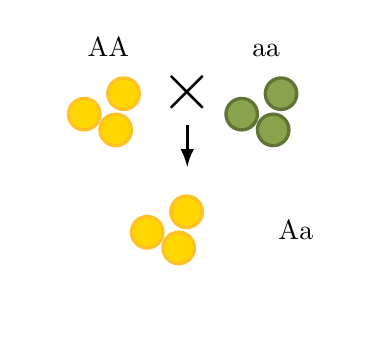
\begin{tikzpicture}
  \node[label={[label distance=-0.5cm]90:AA}] (p1) at (0, 0){\peas{\peaYellow}{\peaYellowOutl}{0.2}{5}};
  \node (x) at (1, 0.25){\Huge{$\times$}};
  \node[label={[label distance=-0.5cm]90:aa}] (p2) at (2, 0){\peas{\peaGreen}{\peaGreenOutl}{0.2}{5}};
  \node[label={[label distance=0.2cm]0:Aa}] (f1) at (0.8, -1.5){\peas{\peaYellow}{\peaYellowOutl}{0.2}{5}};
  \draw[->, very thick] (x) --(1, -0.7);
  \end{tikzpicture}
  \vspace{-0.5cm}\\
Mendel observed some traits were ``hidden''
\begin{itemize}
  \item reappeared when recombined
  \item inheritance of factors, i.e. ``genes''
\end{itemize}
\end{column}

\begin{column}{0.6\linewidth}

  \begin{center}
     \begin{tabular}{cc}
      & \hspace{1cm} \peas{\peaYellow}{\peaYellowOutl}{0.2}{1} \\ 
      \peas{\peaYellow}{\peaYellowOutl}{0.2}{1} \hspace{-0.5cm}  & \begin{tabular}{l|c|c|}
       \multicolumn{1}{c}{} & \multicolumn{1}{c}{\Huge{$A$}} & \multicolumn{1}{c}{\Huge{$a$}} \\ \cline{2-3} 
       \Huge{$A$} & \peas{\peaYellow}{\peaYellowOutl}{0.2}{5} & \peas{\peaYellow}{\peaYellowOutl}{0.2}{5}  \\ \cline{2-3} 
       \Huge{$a$} & \peas{\peaYellow}{\peaYellowOutl}{0.2}{5} & \peas{\peaGreen}{\peaGreenOutl}{0.2}{5} \\ \cline{2-3} 
      \end{tabular}
  \end{tabular}
  \end{center}
\end{column}
\end{columns}
}

\frame{\frametitle{``Incomplete'' Dominance}
  \begin{columns}
\begin{column}{0.4\linewidth}
  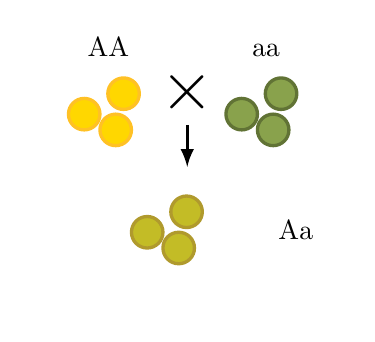
\begin{tikzpicture}
  \node[label={[label distance=-0.5cm]90:AA}] (p1) at (0, 0){\peas{\peaYellow}{\peaYellowOutl}{0.2}{5}};
  \node (x) at (1, 0.25){\Huge{$\times$}};
  \node[label={[label distance=-0.5cm]90:aa}] (p2) at (2, 0){\peas{\peaGreen}{\peaGreenOutl}{0.2}{5}};
  \node[label={[label distance=0.2cm]0:Aa}] (f1) at (0.8, -1.5){\peas{\peaBtwn}{\peaBtwnOutl}{0.2}{5}};
  \draw[->, very thick] (x) --(1, -0.7);
  \end{tikzpicture}
  \vspace{-0.5cm}\\
Not true for all traits
\begin{itemize}
  \item some seemed to blend
\end{itemize}
\end{column}

\begin{column}{0.6\linewidth}

  \begin{center}
     \begin{tabular}{cc}
      & \hspace{1cm} \peas{\peaYellow}{\peaYellowOutl}{0.2}{1} \\ 
     \peas{\peaYellow}{\peaYellowOutl}{0.2}{1} \hspace{-0.5cm}  & \begin{tabular}{l|c|c|}
       \multicolumn{1}{c}{} & \multicolumn{1}{c}{\Huge{$A$}} & \multicolumn{1}{c}{\Huge{$a$}} \\ \cline{2-3} 
       \Huge{$A$} & \peas{\peaYellow}{\peaYellowOutl}{0.2}{5} & \peas{\peaBtwn}{\peaBtwnOutl}{0.2}{5} \\ \cline{2-3} 
       \Huge{$a$} & \peas{\peaBtwn}{\peaBtwnOutl}{0.2}{5} & \peas{\peaGreen}{\peaGreenOutl}{0.2}{5} \\ \cline{2-3} 
      \end{tabular}
  \end{tabular}
  \end{center}

\end{column}
\end{columns}
}


\section{Quantitative Genetics}
\frame{\frametitle{Two waring sides}

\begin{columns}

\begin{column}{0.3\linewidth}
\centering
Mendelians\\

\vspace{3mm}

\includegraphics[width=0.6\linewidth]{Bateson}

William Bateson
\end{column}


\begin{column}{0.4\linewidth}
\visible<2->{
\centering
Quantitative Genetics\\ is born

\includegraphics[width=0.6\linewidth]{"\string~/Dropbox/PLBRG2010_2017/ModelsInBreedingLecture/Fisher"}

Ronald Fisher

}
\end{column}

\begin{column}{0.3\linewidth}
\centering
Biometricians\\ 

\vspace{3mm}

\includegraphics[width=0.6\linewidth]{Pearson}

Karl Pearson
\end{column}

\end{columns}

\vspace{5mm}
\visible<3>{
  
\begin{itemize}
  \item 1918. The Correlation between Relatives on the Supposition of Mendelian Inheritance
  \item Used Mendelian genetics to explain continuous variation
\end{itemize}
}

%  \begin{itemize}
%     \item Multi gene inheritance
%     \item Genetic variance
%     \item Coefficient of ancestry
%   \end{itemize}
% \vspace{2mm}
% Allow for ``Incomplete'' dominance, known as ``Additive''
}


% \begin{columns}

% \begin{column}{0.5\linewidth}
% \centering
% Ronald Fisher
% \includegraphics[width=0.6\linewidth]{"\string~/Dropbox/PLBRG2010_2017/ModelsInBreedingLecture/Fisher"}   
% \end{column}

% \begin{column}{0.33\linewidth}
% \begin{center}
% J.B.S. Haldane

% \includegraphics[width=0.6\linewidth]{"\string~/Dropbox/PLBRG2010_2017/ModelsInBreedingLecture/Haldane"}
% \end{center}
% \end{column}

% \begin{column}{0.33\linewidth}
% \begin{center}
% Sewall Wright

% \includegraphics[width=0.6\linewidth]{"\string~/Dropbox/PLBRG2010_2017/ModelsInBreedingLecture/Wright"}
% \end{center}
% \end{column}
% \end{columns}

% \vspace{5mm}

% Used Mendelian genetics to explain continuous variation (biometry)
%  \begin{itemize}
%     \item Multi gene inheritance
%     \item Genetic variance
%     \item Coefficient of ancestry
%   \end{itemize}
% \vspace{2mm}
% % Allow for ``Incomplete'' dominance, known as ``Additive''
  
% }


% compare Qual and quant
\frame{\frametitle{Qualitative vs Quantitative traits}
 
\begin{columns}

\begin{column}{0.5\linewidth}
 \begin{itemize}
  \item Qualitative traits 
    \begin{itemize}
     \item yellow / green
     \item tall / short
     \item early / late
     \item high / low yielding
    \end{itemize}
  \end{itemize}

\end{column}


\begin{column}{0.5\linewidth}
 \begin{itemize}
    \item Quantitative traits 
     \begin{itemize}
     \item chlorophyll (g)
     \item plant height (cm)
     \item days to flowering 
     \item bushels acre$^{-1}$
     \end{itemize}
  \end{itemize}

\end{column}

\end{columns}
\vspace{1cm}
We will treat the genetics of continuous traits as a (linear) mathematical problem!
}


\subsection{Punnet Squares Additive}
% \frame{\frametitle{``Complete'' Dominance}
%   \begin{center}
%      \begin{tabular}{cc}
%       & \hspace{1cm} \wheats{0}{5}{7.5}{0.2}{2} \\ 
%      \wheats{0}{5}{7.5}{0}{2} & \begin{tabular}{l|c|c|}
%        \multicolumn{1}{c}{} & \multicolumn{1}{c}{\Huge{$A$}} & \multicolumn{1}{c}{\Huge{$a$}} \\ \cline{2-3} 
%        \Huge{$A$} & \wheats{0}{5}{7.5}{0.2}{2} & \wheats{0}{5}{7.5}{0.2}{2}  \\ \cline{2-3} 
%        \Huge{$a$} & \wheats{0}{5}{7.5}{0.2}{2} & \wheats{5}{5}{2.5}{0.2}{2} \\ \cline{2-3} 
%       \end{tabular}
%   \end{tabular}
%   \end{center}
% }

\frame{\frametitle{Additive Single Locus}
Additive effects increase linearly with the total number of alleles

\vspace{5mm}

%   \begin{center}
%   \begin{tabular}{l|c|c|}
%        \multicolumn{1}{c}{} & \multicolumn{1}{c}{\Huge{$A$}} & \multicolumn{1}{c}{\Huge{$a$}} \\ \cline{2-3} 
%        \Huge{$A$} & \wheats{0}{3.5}{8.25}{0}{2} &  \wheats{3.25}{3.5}{5.25}{0}{2} \\ \cline{2-3} 
%        \Huge{$a$} & \wheats{3.25}{3.5}{5.25}{0}{2} & \wheats{6.25}{3.5}{2.5}{0}{2} \\ \cline{2-3} 
%   \end{tabular}
% \end{center}
% }

\begin{center}
  \begin{tabular}{l|c|c|}
       \multicolumn{1}{c}{} & \multicolumn{1}{c}{\Huge{$A$}} & \multicolumn{1}{c}{\Huge{$a$}} \\ \cline{2-3} 
       \Huge{$A$} & \largeWheat{9mm}{2} &  \mediumWheat{9mm}{2} \\ \cline{2-3} 
       \Huge{$a$} & \mediumWheat{9mm}{2} & \smallWheat{9mm}{2} \\ \cline{2-3} 
  \end{tabular}
\end{center}
}

% \frame{\frametitle{Additive Two Loci}
%   \begin{center}
%   \begin{tabular}{l|c|c|c|c|}
%        \multicolumn{1}{c}{} & \multicolumn{1}{c}{\Huge{$AB$}} & \multicolumn{1}{c}{\Huge{$aB$}} & \multicolumn{1}{c}{\Huge{$Ab$}} & \multicolumn{1}{c}{\Huge{$ab$}} \\ \cline{2-5} 
%        \Huge{$AB$} & \wheats{0}{3.5}{8.25}{0}{1.4} &  \wheats{1.75}{3.5}{6.75}{0}{1.4} & \wheats{1.75}{3.5}{6.75}{0}{1.4} &  \wheats{3.25}{3.5}{5.25}{0}{1.4} \\ \cline{2-5} 
%        \Huge{$aB$} & \wheats{1.75}{3.5}{6.75}{0}{1.4} & \wheats{3.25}{3.5}{5.25}{0}{1.4} & \wheats{3.25}{3.5}{5.25}{0}{1.4} & \wheats{4.75}{3.5}{3.75}{0}{1.4} \\ \cline{2-5} 
%        \Huge{$Ab$} & \wheats{1.75}{3.5}{6.75}{0}{1.4} &  \wheats{3.25}{3.5}{5.25}{0}{1.4} & \wheats{3.25}{3.5}{5.25}{0}{1.4} &  \wheats{4.75}{3.5}{3.75}{0}{1.4} \\ \cline{2-5} 
%        \Huge{$ab$} & \wheats{3.25}{3.5}{5.25}{0}{1.4} & \wheats{4.75}{3.5}{3.75}{0}{1.4} & \wheats{4.75}{3.5}{3.75}{0}{1.4} & \wheats{6.25}{3.5}{2.25}{0}{1.4} \\ \cline{2-5} 
%   \end{tabular}
% \end{center}
% }



\subsection{Single Locus Model}



% \frame{\frametitle{The Single Locus Model}

%   \[ y_ij = \mu + G_i + E_j + e_ij\]

% \begin{center}
% \textbf{Phenotype = Genotype + Environment} + error
% \end{center}

% \begin{itemize}
%   \item Genotype = $G_i$ = genetic effect of the $i^\text{th}$ individual 
%   \item Environment = $E_j$ = effect of the $j^\text{th}$ environment
%   \item error = $e_ij$ = some error
% \end{itemize}



% \frame{\frametitle{The Single Locus Model}

% \begin{center}
% \textbf{Phenotype = Genotype} + error
% \end{center}
% \pause

%   \[ y_{ij} = \mu + G_i + e_{ij}\]

% \begin{itemize}
%   \item Genotype = $G_i$ = genetic effect of the $i^\text{th}$ individual 
%   \item error = $e_{ij}$ = some error
% \end{itemize}

% \vspace{5mm}

% \pause

% We will begin with the assumption that only one locus effects our phenotype
% }



\frame{\frametitle{The Single Locus Model}

\begin{center}
\textbf{Phenotype = Genotype} + Environment
\end{center}
\pause

  \[ y_{ij} = G_i + e_{ij}\]

\begin{itemize}
  \item Genotype = $G_i$ = genetic effect of the $i^\text{th}$ individual 
  \item residual = $e_{ij}$ = some deviation from the genetic effect
\end{itemize}

\vspace{5mm}

\pause

We will begin with the assumption that only one locus effects our phenotype
}

\frame{\frametitle{The Single Locus Model II - Matrix notation}

\begin{tabular}{ll}
% \smallWheat{1cm}{1} $= aa$ \\
\largeWheat{0.6cm}{1} $= AA$ \hspace{3cm} & \visible<2->{$y_1 = x_1 \beta_a + e_1$} \\
\mediumWheat{0.6cm}{1} $= Aa$ \hspace{3cm} & \visible<2->{$y_2 = x_2 \beta_a + e_2$} \\
\smallWheat{0.6cm}{1} $= aa$ \hspace{3cm} & \visible<2->{$y_3 = x_3 \beta_a + e_3$} \\
% \largeWheat{1cm}{1} $= AA$
\end{tabular}

% \pause


\vspace{1mm}
\visible<3>{
\[\mathbf{y} = \mathbf{x}_a \beta_a + \mathbf{e}\]
\begin{equation*}
\begin{bmatrix}
  y_1\\      
  y_2\\
  y_3\\
  \vdots\\
  y_n
\end{bmatrix}
=  \begin{bmatrix}
  aa\\
  Aa\\
  Aa\\
  \vdots\\
  AA
\end{bmatrix}
\begin{bmatrix}
  \beta_a
\end{bmatrix}
+
\begin{bmatrix}
  e_1\\
  e_2\\
  e_3\\
  \vdots\\
  e_n
\end{bmatrix}
\pause
= \begin{bmatrix}
  0\\
  1\\
  1\\
  \vdots\\
  2
\end{bmatrix}
\begin{bmatrix}
  \beta_a
\end{bmatrix}
+
\begin{bmatrix}
  e_1\\
  e_2\\
  e_3\\
  \vdots\\
  e_n
\end{bmatrix}
\end{equation*}
}
% % \pause
% \centering
% \highlite{But what about dominance?}


}

\frame{\frametitle{The Single Locus Model III - Dominance}

\[\mathbf{y} = \mathbf{x}_a \beta_a + \mathbf{x}_d \beta_d + \mathbf{e}\]

\vspace{5mm}

\begin{equation*}
\begin{bmatrix}
  y_1\\      
  y_2\\
  y_3\\
  \vdots\\
  y_n
\end{bmatrix}
= \begin{bmatrix}
  aa & \text{hom}\\
  Aa & \text{het}\\
  Aa & \text{het}\\
  \vdots & \vdots\\
  AA & \text{hom}
\end{bmatrix}
\begin{bmatrix}
  \beta_a\\
  \beta_d
\end{bmatrix}
+
\begin{bmatrix}
  e_1\\
  e_2\\
  e_3\\
  \vdots\\
  e_n
\end{bmatrix}
\pause
= \begin{bmatrix}
  0 & 0\\
  1 & 1\\
  1 & 1\\
  \vdots & \vdots\\
  2 & 0
\end{bmatrix}
\begin{bmatrix}
  \beta_a\\
  \beta_d
\end{bmatrix}
+
\begin{bmatrix}
  e_1\\
  e_2\\
  e_3\\
  \vdots\\
  e_n
\end{bmatrix}
\end{equation*}

\pause

Lets see how this works...
}

% \frame{\frametitle{The Single Locus Model}

%   \[ y_{ij} = \mu + xa_i \beta a_i + xd_i \beta d_i + e_{ij}\]

% \[\mathbf{y} = \mathbf{1} \mu + \mathbf{Zg} + \mathbf{e}\]
% \[\mathbf{y} = \mathbf{X} \boldsymbol \beta + \mathbf{Zg} + \mathbf{e}\]

% }

\frame{\frametitle{Additive only}
   \centering
   
    \includegraphics<1>[width = 0.8\linewidth, page=1]{"\string~/Dropbox/PLBRG2010_2017/ModelsInBreedingLecture/addFig"}%
    \includegraphics<2>[width = 0.8\linewidth, page=2]{"\string~/Dropbox/PLBRG2010_2017/ModelsInBreedingLecture/addFig"}%
    \includegraphics<3>[width = 0.8\linewidth, page=3]{"\string~/Dropbox/PLBRG2010_2017/ModelsInBreedingLecture/addFig"}%
    \includegraphics<4>[width = 0.8\linewidth, page=4]{"\string~/Dropbox/PLBRG2010_2017/ModelsInBreedingLecture/addFig"}%
    \includegraphics<5>[width = 0.8\linewidth, page=5]{"\string~/Dropbox/PLBRG2010_2017/ModelsInBreedingLecture/addFig"}%
    \includegraphics<6>[width = 0.8\linewidth, page=6]{"\string~/Dropbox/PLBRG2010_2017/ModelsInBreedingLecture/addFig"}%
 }



\frame{\frametitle{Additive with Dominance}
   \centering
   
    \includegraphics<1>[width = 0.8\linewidth, page=1]{"\string~/Dropbox/PLBRG2010_2017/ModelsInBreedingLecture/domFig"}%
    \includegraphics<2>[width = 0.8\linewidth, page=2]{"\string~/Dropbox/PLBRG2010_2017/ModelsInBreedingLecture/domFig"}%
    \includegraphics<3>[width = 0.8\linewidth, page=3]{"\string~/Dropbox/PLBRG2010_2017/ModelsInBreedingLecture/domFig"}%
    \includegraphics<4>[width = 0.8\linewidth, page=4]{"\string~/Dropbox/PLBRG2010_2017/ModelsInBreedingLecture/domFig"}%
    \includegraphics<5>[width = 0.8\linewidth, page=5]{"\string~/Dropbox/PLBRG2010_2017/ModelsInBreedingLecture/domFig"}%
    \includegraphics<6>[width = 0.8\linewidth, page=6]{"\string~/Dropbox/PLBRG2010_2017/ModelsInBreedingLecture/domFig"}%
 }


% \frame{\frametitle{Additive only}
%   \begin{center}
%     \includegraphics<1>[width = 0.6\linewidth, page=1]{"\string~/Dropbox/PLBRG2010_2017/ModelsInBreedingLecture/singleLocus"} 
%     \includegraphics<3>[width = 0.6\linewidth, page=2]{"\string~/Dropbox/PLBRG2010_2017/ModelsInBreedingLecture/singleLocus"} 

%     \includegraphics<2>[width = 0.6\linewidth, page=1]{"\string~/Dropbox/PLBRG2010_2017/ModelsInBreedingLecture/singleLocusFit"} 
%     \includegraphics<4>[width = 0.6\linewidth, page=2]{"\string~/Dropbox/PLBRG2010_2017/ModelsInBreedingLecture/singleLocusFit"} 
%   \end{center}
% }

% \frame{\frametitle{Pure Dominance}
%   \begin{center}
%     \includegraphics<1>[width = 0.6\linewidth, page=3]{"\string~/Dropbox/PLBRG2010_2017/ModelsInBreedingLecture/singleLocus"} 
%     \includegraphics<3>[width = 0.6\linewidth, page=4]{"\string~/Dropbox/PLBRG2010_2017/ModelsInBreedingLecture/singleLocus"} 

%     \includegraphics<2>[width = 0.6\linewidth, page=3]{"\string~/Dropbox/PLBRG2010_2017/ModelsInBreedingLecture/singleLocusFit"} 
%     \includegraphics<4>[width = 0.6\linewidth, page=4]{"\string~/Dropbox/PLBRG2010_2017/ModelsInBreedingLecture/singleLocusFit"} 
%   \end{center}
% }

% \subsection{Over-Dominance}
% \frame{\frametitle{Over-Dominance}

% Ok, so what about that hybrid vigor we always talk about?

% \vspace{5mm}

%   \begin{center}
%   \begin{tabular}{l|c|c|}
%        \multicolumn{1}{c}{} & \multicolumn{1}{c}{\Huge{$A$}} & \multicolumn{1}{c}{\Huge{$a$}} \\ \cline{2-3} 
%        \Huge{$A$} & \mediumWheat{5mm}{2} & \largeWheat{5mm}{2}  \\ \cline{2-3} 
%        \Huge{$a$} & \largeWheat{5mm}{2} & \smallWheat{5mm}{2} \\ \cline{2-3} 
%   \end{tabular}
% \end{center}
% }

% \frame{\frametitle{Over-Dominance}
%   \begin{center}
%     \includegraphics<1>[width = 0.6\linewidth, page=5]{"\string~/Dropbox/PLBRG2010_2017/ModelsInBreedingLecture/singleLocus"} 
%     \includegraphics<3>[width = 0.6\linewidth, page=6]{"\string~/Dropbox/PLBRG2010_2017/ModelsInBreedingLecture/singleLocus"} 

%     \includegraphics<2>[width = 0.6\linewidth, page=5]{"\string~/Dropbox/PLBRG2010_2017/ModelsInBreedingLecture/singleLocusFit"} 
%     \includegraphics<4>[width = 0.6\linewidth, page=6]{"\string~/Dropbox/PLBRG2010_2017/ModelsInBreedingLecture/singleLocusFit"} 
%   \end{center}
% }
% Additive vairance, dominance variance
% heritable variability


% \frame{\frametitle{Lets simulate it}

% Let's start with the single locus:
% \textit{https://nsantantonio.shinyapps.io/singlelocus/}

% \vspace{3cm}
% \visible<2>{\textit{https://nsantantonio.shinyapps.io/quantitative/}}

% }

\frame{\frametitle{Lets simulate it}

Let's start with the single locus:
\href{https://nsantantonio.shinyapps.io/singlelocus/}{nsantantonio.shinyapps.io/singlelocus/}

% \vspace{3cm}

% \visible<2>{\href{https://nsantantonio.shinyapps.io/quantitative/}{nsantantonio.shinyapps.io/quantitative/}}
}


\subsection{Genetic Variance}
\frame{\frametitle{Genetic Variance}
  \begin{tabular}{l}
  Let $n =$ number of individuals \\
  Let P = frequency of AA's \\
  Let 2Q = frequency of Aa's \\
  Let R = frequency of aa's \\
  \end{tabular} such that $P + 2Q + R = 1$

\begin{align*}
  \text{E}[\mathbf{x}] &= \frac{1}{n}\sum_{i = 1}x_i \\
  \mu &= Pa + 2Qd - Ra \\[2em]
  % 0 &= P(a-m) + 2Q(d-m) - R(a-m) 
% \end{align*}
% \vspace{5mm}
% \begin{align*}
  \text{Var}(\mathbf{x}) &= \frac{1}{n}\sum_{i=1} (x_i - \mu)^2 \\
    &= P(a-\mu)^2 + 2Q(d-\mu)^2 - R(a-\mu)^2 
\end{align*}

}


\subsection{Genetic Variance}
\frame{\frametitle{Genetic Variance}
  Breeder's Equation:
  \[ \Delta_R = \frac{ir \sigma_a}{c}\]
  \pause
  \vspace{-5mm}
  \begin{center}
    \includegraphics[width = 0.7\linewidth]{"\string~/Dropbox/PLBRG2010_2017/ModelsInBreedingLecture/additiveDominanceVariancePlot"} 
  \end{center}


}

\section{Causal Variants}









\subsection{Mapping}

\frame{\frametitle{Finding causal genes}

\begin{columns}
\begin{column}{0.3\linewidth}
\includegraphics<3->[width = 0.9\linewidth]{"\string~/Dropbox/PLBRG2010_2017/ModelsInBreedingLecture/chrom2_2"} 
\end{column}

\begin{column}{0.7\linewidth}
How do we find causal genes / variants?

\pause

DNA markers!
\begin{itemize}
  \item genotype individuals with genome-wide markers
  \item statistical association between marker and trait
  \begin{itemize}
    \item $H_0: \beta_a = 0$ and $\beta_d = 0$
    \item $H_0: \beta_a \neq 0$ or $\beta_d \neq 0$
  \end{itemize}
  %   \begin{itemize}
  %   \item $\Rightarrow$ Correlate genotype to phenotype!
  % \end{itemize}
  \end{itemize}

\pause
Bi-parental mapping populations 

\begin{itemize}
  \item maximize allele frequencies 
  \begin{itemize}
    \item  Statistical power
  \end{itemize}
\pause
  \item maximize linkage  
  \begin{itemize}
  \item  poor precision... 
  \end{itemize}
\end{itemize}
\end{column}
\end{columns}
}

\subsection{GWAS}

\frame{\frametitle{Genome-Wide Association Studies}
Association Mapping Population 
\begin{itemize}
\item Take advantage of historical recombination events (low linkage)
\pause
\item However, more closely related individuals will share functional alleles, as well as \emph{many} other alleles
\end{itemize}
\vspace{-6mm}
\begin{center}
\includegraphics[width = 0.7\linewidth]{"\string~/Dropbox/MasterGenotypeswithOHMI/HtmanhattanNOCORRECT"} 
\end{center}
}


\frame{\frametitle{Population Structure Problem}
Population structure ``inflates'' significance. Correct with kinship.
\begin{center}
\includegraphics[width = 0.6\linewidth]{"\string~/Dropbox/PLBRG2010_2017/ModelsInBreedingLecture/Heatmap_Kinship"} 
\end{center}
}

\frame{\frametitle{Finding causal genes}

Population structure ``inflates'' significance.
\begin{center}
\includegraphics<1>[width = 0.7\linewidth]{"\string~/Dropbox/MasterGenotypeswithOHMI/HtmanhattanNOCORRECT"} 
\includegraphics<2>[width = 0.7\linewidth]{"\string~/Dropbox/MasterGenotypeswithOHMI/PHmanhattanCR"} 
\includegraphics<3>[width = 0.7\linewidth]{"\string~/Dropbox/MasterGenotypeswithOHMI/PHmanhattan"} 
\includegraphics<4>[width = 0.7\linewidth]{"\string~/Dropbox/MasterGenotypeswithOHMI/GYmanhattan"} 
\end{center}
}

% \frame{\frametitle{Additive Two Loci}
% \begin{center}
%   \begin{tabular}{l|c|c|c|c|}
% \multicolumn{1}{c}{} & \multicolumn{1}{c}{\tiny{$AB$}} & \multicolumn{1}{c}{\tiny{$aB$}} & \multicolumn{1}{c}{\tiny{$Ab$}} & \multicolumn{1}{c}{\tiny{$ab$}} \\ \cline{2-5} 
%        \Huge{$A$} & \largeWheat{9mm}{2} &  \mediumWheat{9mm}{2} & \largeWheat{9mm}{2} &  \mediumWheat{9mm}{2} \\ \cline{2-3} 
%        \Huge{$a$} & \mediumWheat{9mm}{2} & \smallWheat{9mm}{2} & \largeWheat{9mm}{2} &  \mediumWheat{9mm}{2}\\ \cline{2-3} 
%   \end{tabular}
% \end{center}

% }
% \frame{\frametitle{Additive Two Loci}
%   \begin{center}
%   \begin{tabular}{l|c|c|c|c|}
%        \multicolumn{1}{c}{} & \multicolumn{1}{c}{\tiny{$AB$}} & \multicolumn{1}{c}{\tiny{$aB$}} & \multicolumn{1}{c}{\tiny{$Ab$}} & \multicolumn{1}{c}{\tiny{$ab$}} \\ \cline{2-5} 
%        \tiny{$AB$} & \bigWheat{1mm}{1} & \largeWheat{1mm}{1} & \largeWheat{1mm}{1} & \mediumWheat{1mm}{1}\\ \cline{2-5} 
%        \tiny{$aB$} & \largeWheat{1mm}{1} & \mediumWheat{1mm}{1} & \mediumWheat{1mm}{1} & \smallWheat{1mm}{1} \\ \cline{2-5} 
%        \tiny{$Ab$} & \largeWheat{1mm}{1} & \mediumWheat{1mm}{1} & \mediumWheat{1mm}{1} & \smallWheat{1mm}{1} \\ \cline{2-5} 
%        \tiny{$ab$} & \mediumWheat{1mm}{1} & \smallWheat{1mm}{1} & \smallWheat{1mm}{1} & \tinyWheat{1mm}{1} \\ \cline{2-5} 
%   \end{tabular}
% \end{center}
% }



% \frame{\frametitle{Additive Two Loci}
%   \begin{center}
%   \begin{tabular}{l|c|c|c|c|}
%        \multicolumn{1}{c}{} & \multicolumn{1}{c}{\tiny{$AB$}} & \multicolumn{1}{c}{\tiny{$aB$}} & \multicolumn{1}{c}{\tiny{$Ab$}} & \multicolumn{1}{c}{\tiny{$ab$}} \\ \cline{2-5} 
%        \tiny{$AB$} & \tinyWheat{0.1mm}{0} & a & a & a\\ \cline{2-5} 
%        \tiny{$aB$} & a & a & a & a \\ \cline{2-5} 
%        \tiny{$Ab$} & a & a & a & a \\ \cline{2-5} 
%        \tiny{$ab$} & a & a & a & a \\ \cline{2-5} 
%   \end{tabular}
% \end{center}
% }

\frame{\frametitle{Additive Two Loci}
\centering
\includegraphics[width = 0.7\linewidth]{tempFig} 
}


\frame{\frametitle{Lets see what happens when we have many loci}

Let's start with the single locus:
% \href{https://nsantantonio.shinyapps.io/singlelocus/}{nsantantonio.shinyapps.io/singlelocus/}

% \vspace{3cm}

\href{https://nsantantonio.shinyapps.io/quantitative/}{nsantantonio.shinyapps.io/quantitative/}
}
% \frame{\frametitle{Additive Two Loci}
%   \begin{center}
%   \begin{tabular}{l|c|c|c|c|}
%        \multicolumn{1}{c}{} & \multicolumn{1}{c}{\tiny{$AB$}} & \multicolumn{1}{c}{\tiny{$aB$}} & \multicolumn{1}{c}{\tiny{$Ab$}} & \multicolumn{1}{c}{\tiny{$ab$}} \\ \cline{2-5} 
%        \tiny{$AB$} & \tinyWheat{2mm}{0.1} & \tinyWheat{2mm}{0.1} & \tinyWheat{2mm}{0.1} & \tinyWheat{2mm}{0.1}\\ \cline{2-5} 
%        \tiny{$aB$} & \tinyWheat{2mm}{0.1} & \tinyWheat{2mm}{0.1} & \tinyWheat{2mm}{0.1} & \tinyWheat{2mm}{0.1} \\ \cline{2-5} 
%        \tiny{$Ab$} & \tinyWheat{2mm}{0.1} & \tinyWheat{2mm}{0.1} & \tinyWheat{2mm}{0.1} & \tinyWheat{2mm}{0.1} \\ \cline{2-5} 
%        \tiny{$ab$} & \tinyWheat{2mm}{0.1} & \tinyWheat{2mm}{0.1} & \tinyWheat{2mm}{0.1} & \tinyWheat{2mm}{0.1} \\ \cline{2-5} 
%   \end{tabular}
% \end{center}
% }

% \subsection{many locus example}

% \frame{\frametitle{Break for example}
% Lets break for an example...
% }

% \subsection{mixed models}
% \subsection{Pedigree}
  
% \frame{\frametitle{Using expected relationships}

% \begin{columns}
% \begin{column}{0.7\linewidth}
% \begin{center}
% \begin{tikzpicture}[node distance=0.5cm]

%   \node (A) at (2, 0) {Stander};
%   \node (B) at (1, 2) {MN80-224};
%   \node (C) at (3, 2) {Excel};
%   \node (D) at (0, 4) {Bumper};
%   \node (E) at (4, 4) {MN77-825};
%   \node (F) at (5, 6) {MN72-146};
%   \node (G) at (3, 6) {Robust};
%   \node (H) at (2, 8) {Morex};
%   \node (I) at (4, 8) {Manker};
%   \node (J) at (6, 8) {M28};
%   \node (K) at (4, 9) {$f_{\text{Morex, M28}}=0.5$};

%   \draw [->] (B) -- (A);
%   \draw [->] (C) -- (A);
%   \draw [->] (E) -- (C);
%   \draw [->] (G) -- (C);
%   \draw [->] (G) -- (B);
%   \draw [->] (G) -- (E);
%   \draw [->] (D) -- (B);
%   \draw [->] (D) -- (B);
%   \draw [->] (F) -- (E);
%   \draw [->] (H) -- (G);
%   \draw [->] (I) -- (G);
%   \draw [->] (I) -- (F);
%   \draw [->] (J) -- (F);
%   \draw [->] (K) -- (H);
%   \draw [->] (K) -- (J);
% \end{tikzpicture}
% \end{center}

% \end{column}
% \begin{column}{0.7\linewidth}
% \begin{table}
% \caption{Coefficients of ancestry}
% \begin{tabular}{lcccc}
%   & Morex & Robust & Excel & Stander \\ \hline
% Morex   &   1   &   1/2  & 7/16  &  11/32  \\
% Robust  &       &    1   & 27/32 &  43/64  \\
% Excel   &       &        &   1   &  91/128 \\
% Stander &       &        &       &    1    \\ \hline
% \end{tabular}
% Note: because these are inbred lines, we would multiply these coefficients by the inbreeding coefficient, $f = 2$.
% \end{table}

% \begin{equation}
%   \mathbf{A} = 2 \times \begin{bmatrix}
%   1 & 1/2 & 7/16 & 11/32\\
%   1/2 & 1 & 27/32 & 43/64\\
%   7/16 & 27/32 & 1 & 91/128\\
%   11/32 & 43/64 & 91/128 & 1
% \end{bmatrix}
% \end{equation}

% \end{column}
% \end{columns}

% }



% transition from GWAS to GS using yield!
\section{Genomic Selection}
\subsection{Genomic Prediction}

\frame{\frametitle{Genomic Prediction}

\[ G_i = \sum^m_{i = 1} \mathbf{x}_{a_i} \beta_{a_i} \]


\begin{itemize}
\item Genetic value of an individual is the sum of its allele effects
\item Interestingly, same as modeling kinship between individuals!
\end{itemize}

\begin{equation*} 
   \mathbf{y} = \mathbf{1} \mu + \mathbf{X}\boldsymbol\beta + \mathbf{Zg} + \boldsymbol\varepsilon %\tag{\ref{eq:Gindex}}
\end{equation*}

\begin{itemize}
\item $\mathbf{1}_n\mu$ is the global mean 
\item $\mathbf{X}$ is the design matrix 
\item $\boldsymbol \beta$ is the vector of fixed environmental effects.  
\item $\mathbf{Z}$ is the incidence matrix
\item $\mathbf{g} \sim \mathcal{N}(0, \sigma^2_a \mathbf{K})$, random genetic effects
\item $\mathbf{\boldsymbol \varepsilon} \sim \mathcal{N}(0, \sigma^2 \mathbf{R})$, error 
\end{itemize}
}

% \frame{\frametitle{The mixed model}
\frame{\frametitle{Mixed Model Equations}
\begin{equation*} 
   \mathbf{y} = \mathbf{1} \mu + \mathbf{X}\boldsymbol\beta + \mathbf{Zg} + \boldsymbol\varepsilon %\tag{\ref{eq:Gindex}}
\end{equation*}

\[\begin{bmatrix}
  \hat{\boldsymbol{\beta}}\\      
  \hat{\mathbf{g}}
\end{bmatrix}
  =   
\begin{bmatrix}
  \mathbf{X}^\text{T} \mathbf{R}^{-1} \mathbf{X} & \mathbf{X}^\text{T} \mathbf{R}^{-1}\mathbf{Z}\\
  \mathbf{Z}^\text{T} \mathbf{R}^{-1} \mathbf{X} & \mathbf{Z}^\text{T} \mathbf{R}^{-1} \mathbf{Z} + \mathbf{A}^{-1} \left( \frac{\sigma^2_e}{\sigma^2_g} \right)
\end{bmatrix}^{-1}
\begin{bmatrix}
  \mathbf{X}^\text{T} \mathbf{R}^{-1} \mathbf{y}\\
  \mathbf{Z}^\text{T} \mathbf{R}^{-1} \mathbf{y} \
\end{bmatrix}
\]
}


\frame{\frametitle{Genomic Prediction of Grain Yield}
\begin{center}
\includegraphics[width = 0.65\linewidth]{"\string~/Dropbox/MasterGenotypeswithOHMI/YieldGSplot"} 
\end{center}
}

\frame{\frametitle{Genomic Selection}
% So, who cares??
\pause
  Breeder's Equation:
  \[ \Delta_R = \frac{ir \sigma_a}{c}\]

\pause
  \begin{itemize}
    \item Can select without observing phenotypes!
    % \item Same as ``selecting on seedling leaf color''
    \pause
    \item make crosses in (winter) greenhouse to decrease cycle time ($c$)! 
  \end{itemize}
  \pause
  \centering
  \includegraphics[width = 0.7\linewidth]{"\string~/Dropbox/PLBRG2010_2017/ModelsInBreedingLecture/GS"} 
}
\end{document}
